\documentclass[10pt,twocolumn,a4paper]{article}

% -------------------------------------------------
% Idioma y codificación
% -------------------------------------------------
\usepackage[T1]{fontenc}
\usepackage{lmodern}
\usepackage[english]{babel}

% -------------------------------------------------
% Formato del documento
% -------------------------------------------------
\usepackage[
    top=1.8cm,
    bottom=1.8cm,
    left=1.8cm,
    right=1.8cm,
    columnsep=0.7cm
]{geometry}

\usepackage{microtype}
\usepackage{parskip}

% -------------------------------------------------
% Matemáticas
% -------------------------------------------------
\usepackage{amsmath}
\usepackage{amssymb}
\usepackage{bm}

% -------------------------------------------------
% Figuras y tablas
% -------------------------------------------------
\usepackage{graphicx}
\usepackage{booktabs}
\usepackage{siunitx}

% -------------------------------------------------
% Enlaces y referencias
% -------------------------------------------------
\usepackage[hidelinks]{hyperref}

% Carpeta de imágenes
\graphicspath{{images/}}

% -------------------------------------------------
% Información del documento
% -------------------------------------------------
\title{
    \textbf{Vector-Based Goal Representation\\
    for a Mobile Robot}
}

\author{
    Julio Quejido Barrera\\
    Humanoide Robotik\\
    Julio's Laboratories
}

\date{\today}

% =================================================
\begin{document}
% =================================================

\maketitle

\begin{abstract}
This project introduces fundamental vector operations used in mobile
robot navigation. The positions of a robot and a target are represented as 
two-dimensional vectors. From these positions, the displacement vector, Euclidean distance, 
and normalized direction toward the target are calculated. These operations 
provide the mathematical basis for later motion control, path planning, and 
obstacle avoidance algorithms.
\end{abstract}

\section{Introduction}

The positions of a robot and a target are represented as two-dimensional vectors. 
From these positions, the displacement vector, Euclidean distance, 
and normalized direction toward the target are calculated.

The central idea is that a robot needs to know:

\begin{itemize}
    \item where it is,
    \item where the goal is,
    \item how far away the goal is
    \item and in which direction it should move.
\end{itemize}

In a two-dimensional environment positions are represented using vectors:

\[
\mathbf{p} =
\begin{bmatrix}
x \\
y
\end{bmatrix}
\]

\section{Theoretical Background}

\subsection{Position Vectors}

Define the robot position and goal position as:

\[
\mathbf{p}_R =
\begin{bmatrix}
x_R \\
y_R
\end{bmatrix}
\qquad
\mathbf{p}_G =
\begin{bmatrix}
x_G \\
y_G
\end{bmatrix}
\]

Where:

\begin{itemize}
    \item $p_R$ is the position of the robot,
    \item $p_G$ is the position of the goal.
\end{itemize}

In the experiment:

\[
\mathbf{p}_R =
\begin{bmatrix}
0 \\
0
\end{bmatrix}
\qquad
\mathbf{p}_G =
\begin{bmatrix}
5 \\
5
\end{bmatrix}
\]

\subsection{Vector from the Robot to the Goal}

The displacement vector is calculated by subtracting the 
robot position from the goal position:

\[
\mathbf{v}_{RG} = \mathbf{p}_G - \mathbf{p}_R
\]

\subsection{Euclidean Distance}

The distance between the robot and the goal is calculated using the Euclidean norm:

\begin{equation}
    d = \left\lVert \mathbf{v}_{RG} \right\rVert
    \label{eq:robot_goal_distance_norm}
\end{equation}

\begin{equation}
    d = \sqrt{(x_G - x_R)^2 + (y_G - y_R)^2}
    \label{eq:robot_goal_distance}
\end{equation}

\subsection{Normalized Direction Vector}

The direction toward the goal is obtained by normalizing the displacement vector.
It contains direction information independently of distance:

\begin{equation}
    \hat{\mathbf{v}}_{RG}
    =
    \frac{\mathbf{v}_{RG}}
    {\left\lVert \mathbf{v}_{RG} \right\rVert}
    \label{eq:normalized_robot_goal_vector}
\end{equation}

\section{Methodology}

The procedure was:

\begin{itemize}
    \item Define the robot position as a two-dimensional NumPy array.
    \item Define the goal position.
    \item Subtract both vectors to obtain the robot-to-goal displacement.
    \item Calculate the Euclidean distance.
    \item Normalize the displacement vector.
    \item Display the resulting values.
\end{itemize}

\section{Results}

Figure~\ref{fig:Figure_1} shows the representation of the robot 
position, goal position, and displacement vector.

\begin{figure}[ht]
    \centering
    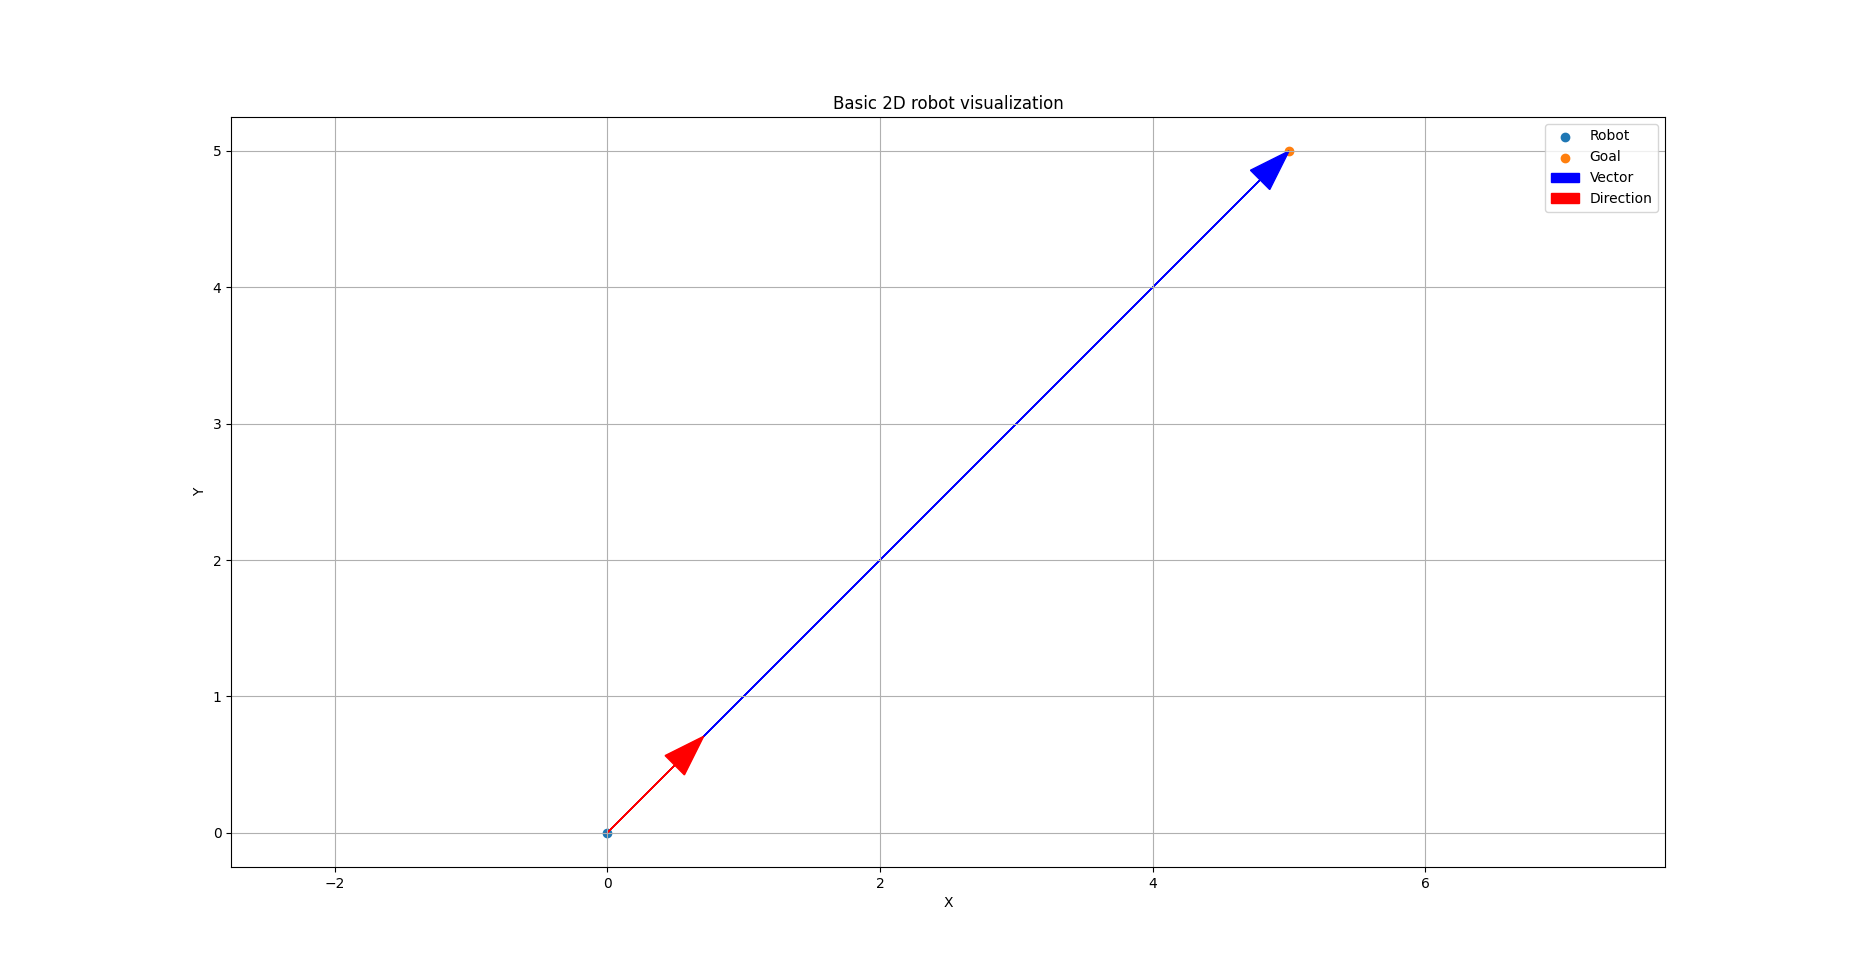
\includegraphics[width=\columnwidth]{Figure_1.png}
    \caption{Two-dimensional representation of the robot}
    \label{fig:Figure_1}
\end{figure}

\begin{align}
    \text{Distance to goal} &= 7.07107, \\
    \text{Direction to goal} &= 
    \begin{bmatrix}
        0.70711 & 0.70711
    \end{bmatrix}.
\end{align}

\section{Project Task}

Represent the robot position
\(\mathbf{p}_R = [0,0]^T\)
and the goal position
\(\mathbf{p}_G = [5,5]^T\)
as NumPy arrays. Compute the vector from the robot to the goal, determine the 
Euclidean distance between both positions, and normalize the displacement vector 
to obtain the direction of motion. Finally, print the calculated values and 
represent the robot, the goal, and the direction vector in a two-dimensional 
graph using Matplotlib.
% =================================================
\end{document}
% =================================================